Während es unmöglich ist, einen Zerfall eines einzelnen Atomkerns vorauszusagen, so ist es bei der Betrachtung einer großen Anzahl von Zerfallsprozessen möglich, statistische Aussagen und Voraussagen über die Gesamtheit der Zerfälle zu treffen. In diesem Versuch wird die Statistik von einer großen Anzahl an radioaktiven Zerfällen eines Präparats mit einem Geiger-Müller-Zählrohr aufgezeichnet und die Statistik der Zerfälle hingehend verschiedener Wahrscheinlichkeitsverteilungen untersucht.

\subsection{Physikalische Grundlagen}

\subsubsection*{Geiger-Müller-Zählrohr}

Ein Geiger-Müller-Zählrohr kann verwendet werden, um verschiedene Arten von Strahlung nachzuweisen. Aufgebaut ist es, wie in \abbref{fig:gm_zaehlrohr} zu sehen, aus einem zylinderförmigen Gehäuse, welches auf der Vorderseite mit einem Fenster versehen und auf der Rückseite geschlossen ist. Am Zählrohr liegt eine Spannung von mehreren 100 bis 1000 Volt an, wobei das Gehäuse selbst als Kathode dient während sich im Gehäuse ein Anodendraht befindet. Das Zählrohr ist mit einem Gas gefüllt, in welchem es bei Kontakt mit einem geladenen Teilchen, welches durch das Fenster in das Zählrohr eindringt, zu einer Ionisation und somit der Erzeugung freier Elektronen kommt. Diese verursachen über eine Gasentladung einen kurzen Stromfluss im Zählrohr, welcher durch eine Schaltung registriert werden kann. 

\begin{figure}[H]
  \centering
  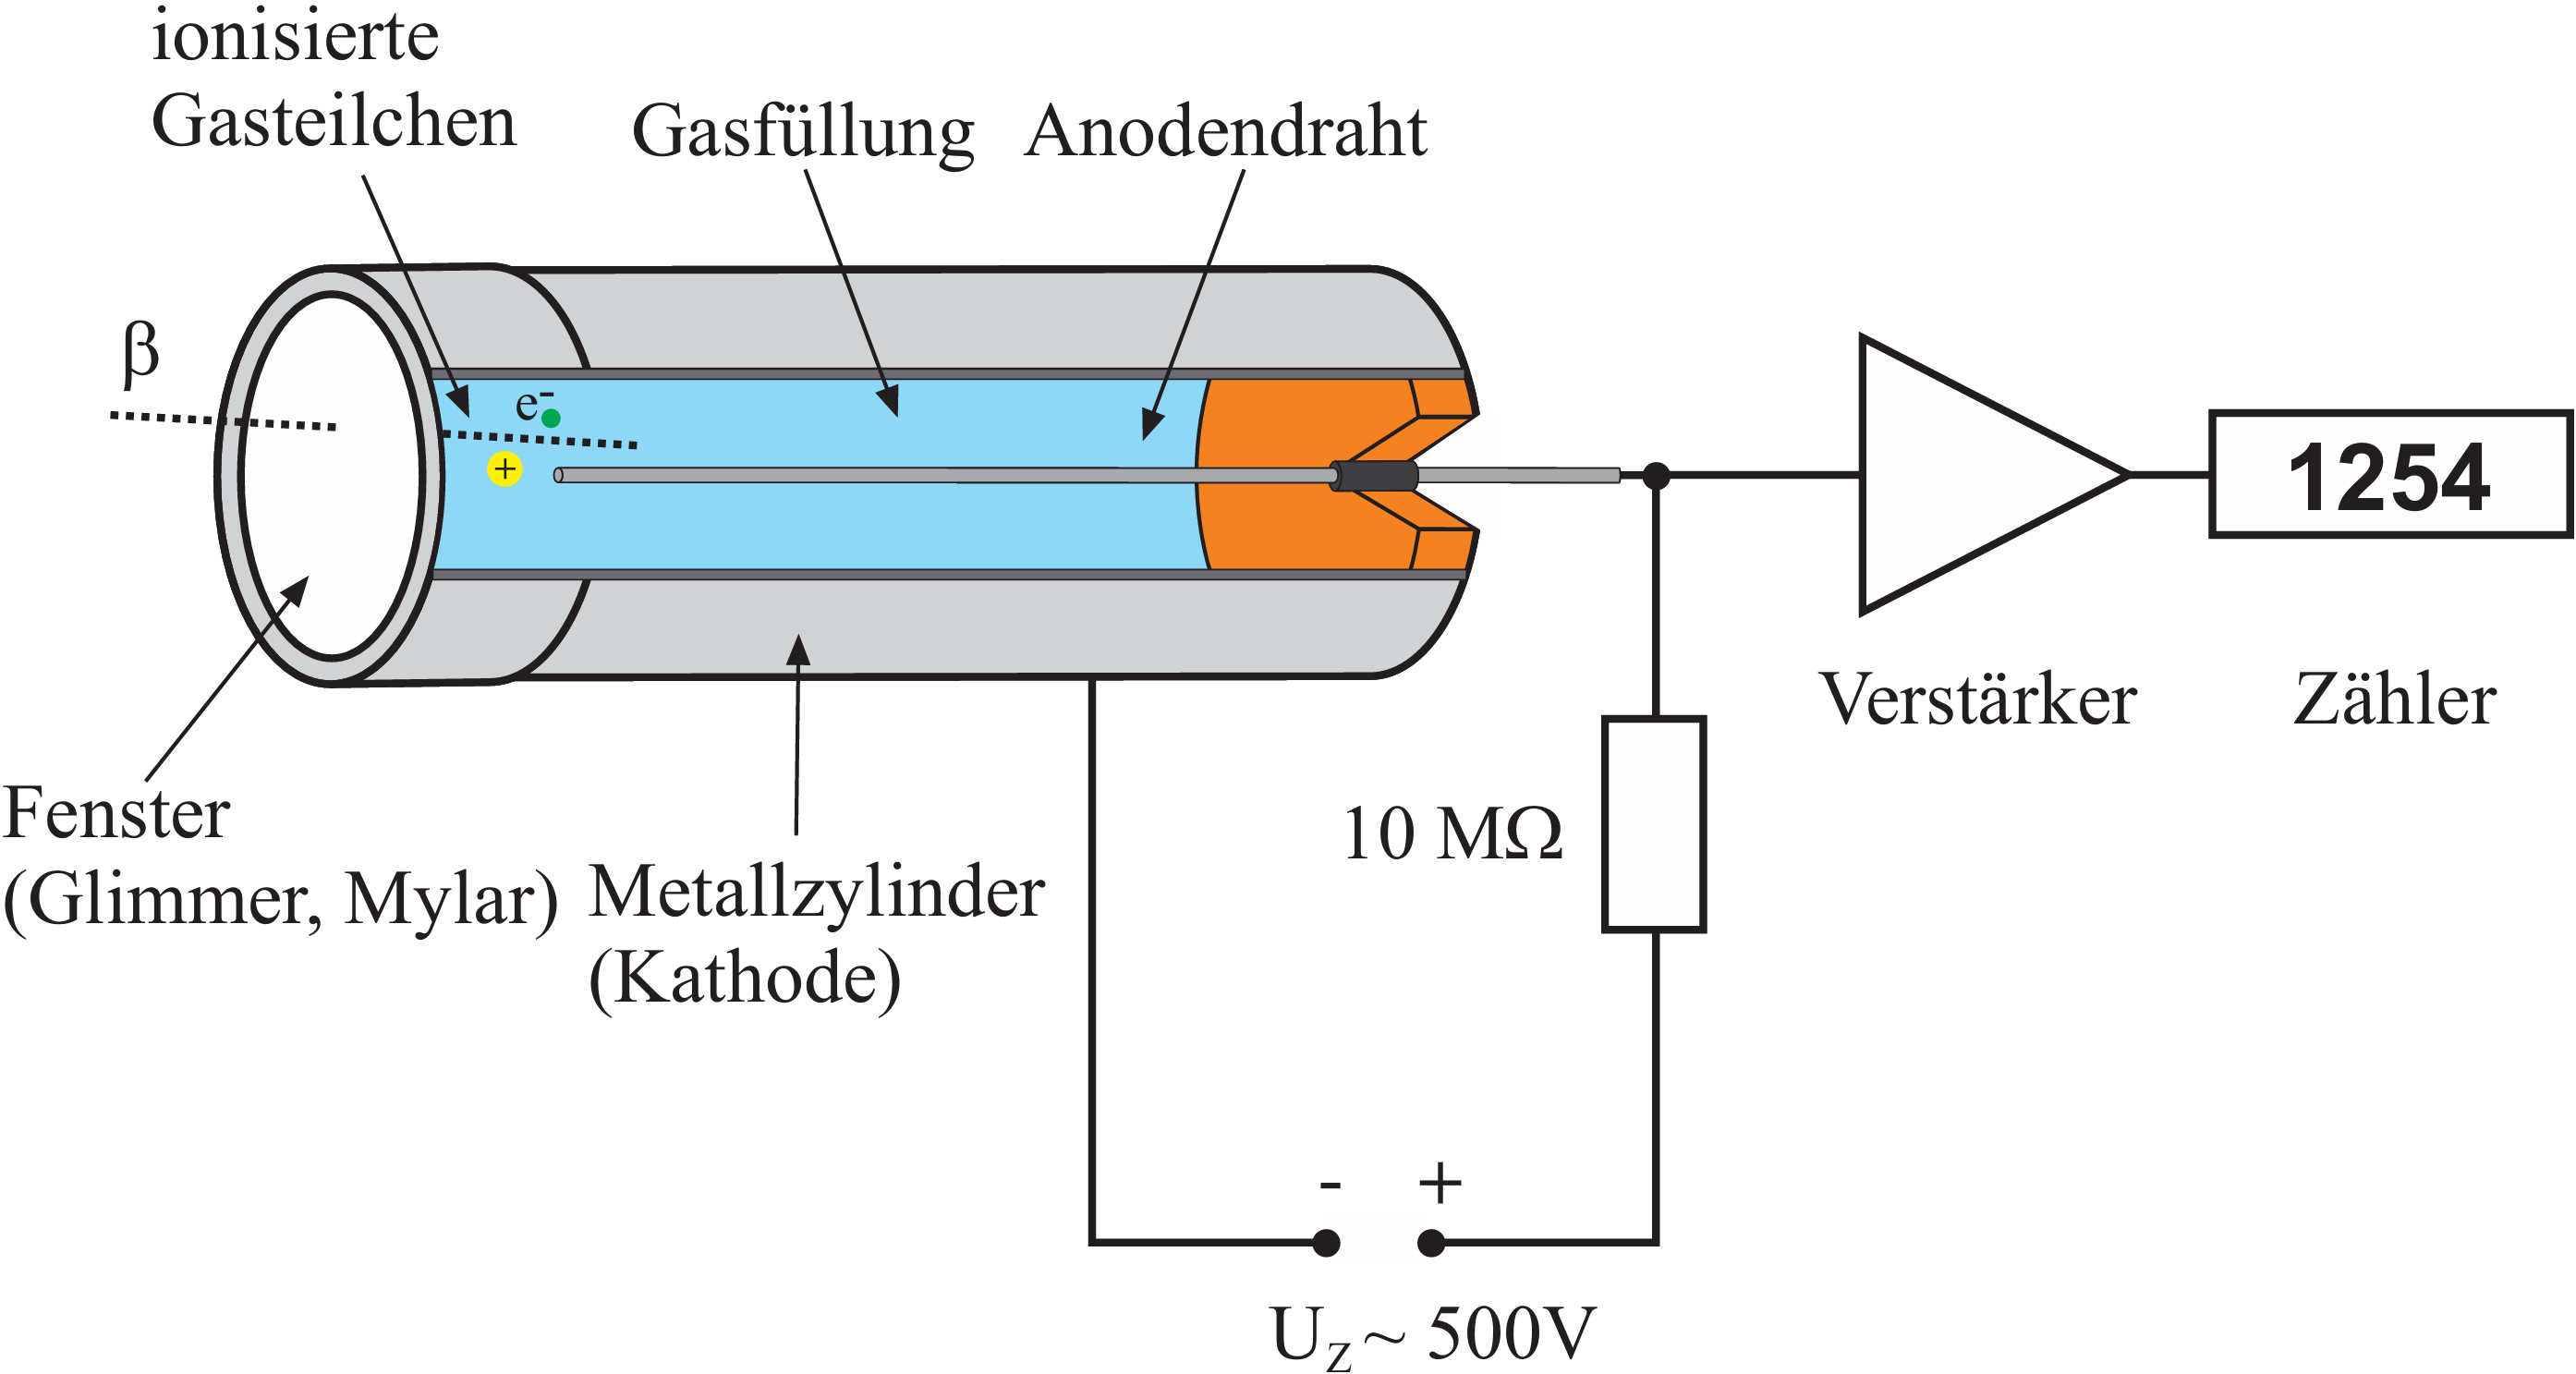
\includegraphics[width=0.8\textwidth]{files/gm_zaehlrohr.png}
  \caption{Schematische Darstellung des Geiger-Müller-Zählrohrs}
  \label{fig:gm_zaehlrohr}
\end{figure}

Für den korrekten Betrieb des Zählrohrs ist die Wahl der anlegten Spannung von großer Bedeutung. Ab einer gewissen Einsatzspannung $U_E$ befindet man sich im sogenannten Plateaubereich. In diesem wird das Zählrohr optimalerweise für das Detektieren von ionisierender Strahlung und Zählanwendungen, wie in diesem Versuch relevant, betrieben. Die Beschleunigung der durch die Ionisation primär erzeugten freien Elektronen ist in hier so hoch, dass diese eine Lawine an propagierenden Ionisationen im Füllgas entlang des Anodendrahts auslösen. Hierdurch wird erzielt, dass jedes eindringende Teilchen, unabhängig von seiner Energie, ein gleich großes Entladungssignal auslöst.

\begin{figure}[H]
  \centering
  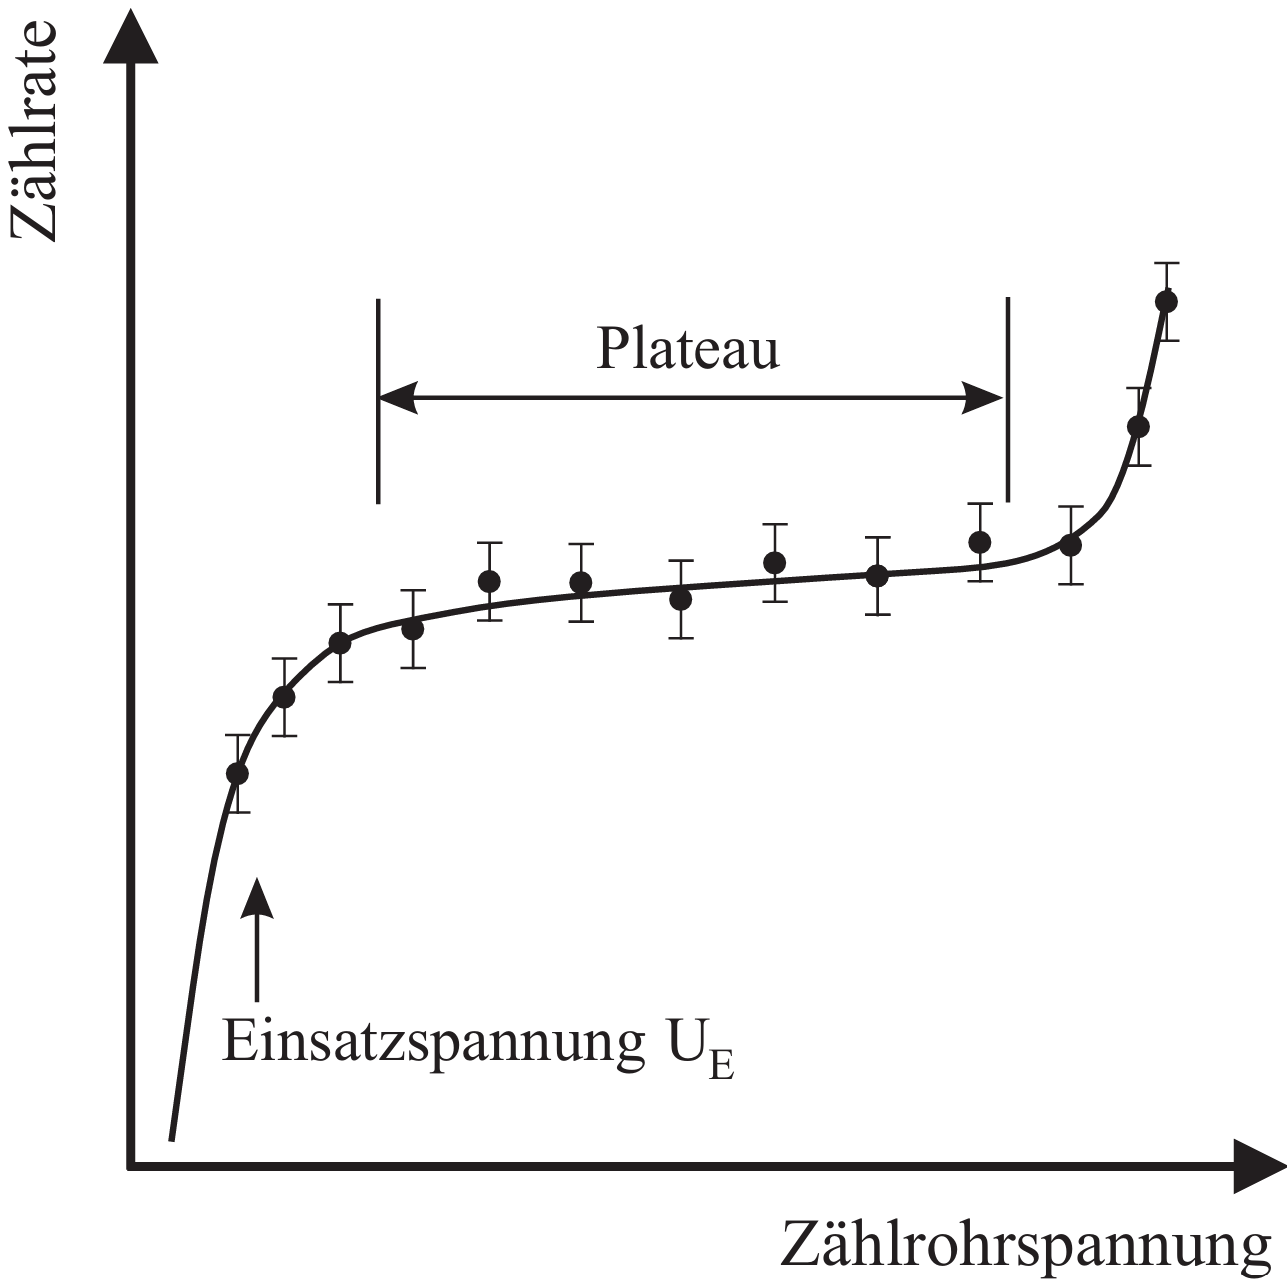
\includegraphics[width=0.4\textwidth]{files/plateaubereich.png}
  \caption{Plateaubereich des Geiger-Müller-Zählrohrs}
  \label{fig:gm_zaehlrohr}
\end{figure}

Die Ermittlung des Plateaubereichs wird hier der erste Teil der Versuchsdurchführung sein.

\subsubsection*{Wahrscheinlichkeitsverteilungen}

Wie im Einleitungstext kurz beschrieben, lassen sich radioaktiven Zerfälle, auch wenn diese im einzelnen komplett zufällig auftreten, in einer Gesamtheit sehr vieler Zerfälle in Form von Wahrscheinlichkeitsverteilungen erfassen, untersuchen und nutzen, um Vorhersagen zu tätigen. Die hierbei relevanten Verteilungen sind die Binomial-, die Poisson- und die Gauss-Verteilung. 

\textbf{Binomialverteilung.} Die Binomialverteilung gibt die Wahrscheinlichkeit dafür an, dass ein Ereignis mit der Eintrittswahrscheinlichkeit $p$ bei $n$ voneinander unabhängigen Versuchen genau $k$ mal eintritt. Die Verteilungsfunktion dieser ist gegeben durch
\begin{align}
  B(k;n,p) = \binom{n}{k} p^k (1 - p)^{n-k}.
\end{align}
Hierbei sind $n, k \in \N$, es handelt sich also um eine diskrete Wahrscheinlichkeitsverteilung. Für die Binomialverteilung gilt
\begin{align}
  \text{Mittelwert: }& \mean{k} = np,\\[0.6em]
  \text{Varianz: }& \sigma^2 = np(1-p).
\end{align}

Übertragaen auf radioaktive Zerfälle beschreibt die Binomialverteilung die Wahrscheinlichkeit, dass von $n$ Atomkernen innerhalb einer Zeit $t$ genau $k$ Kerne zerfallen sind. Hierbei geht die Zeit in die Beschreibung der Wahrscheinlichkeit
\begin{align}
  p(t) = 1 - \e{-\lambda t}
\end{align} 
ein, da zu erwarten ist, dass nach einer längeren Zeit eine größere Anzahl an Zerfällen zu beobachten ist. $\lambda$ ist die für ein Isotop charakteristische Zerfallskonstante.

\begin{figure}[H]
  \centering
  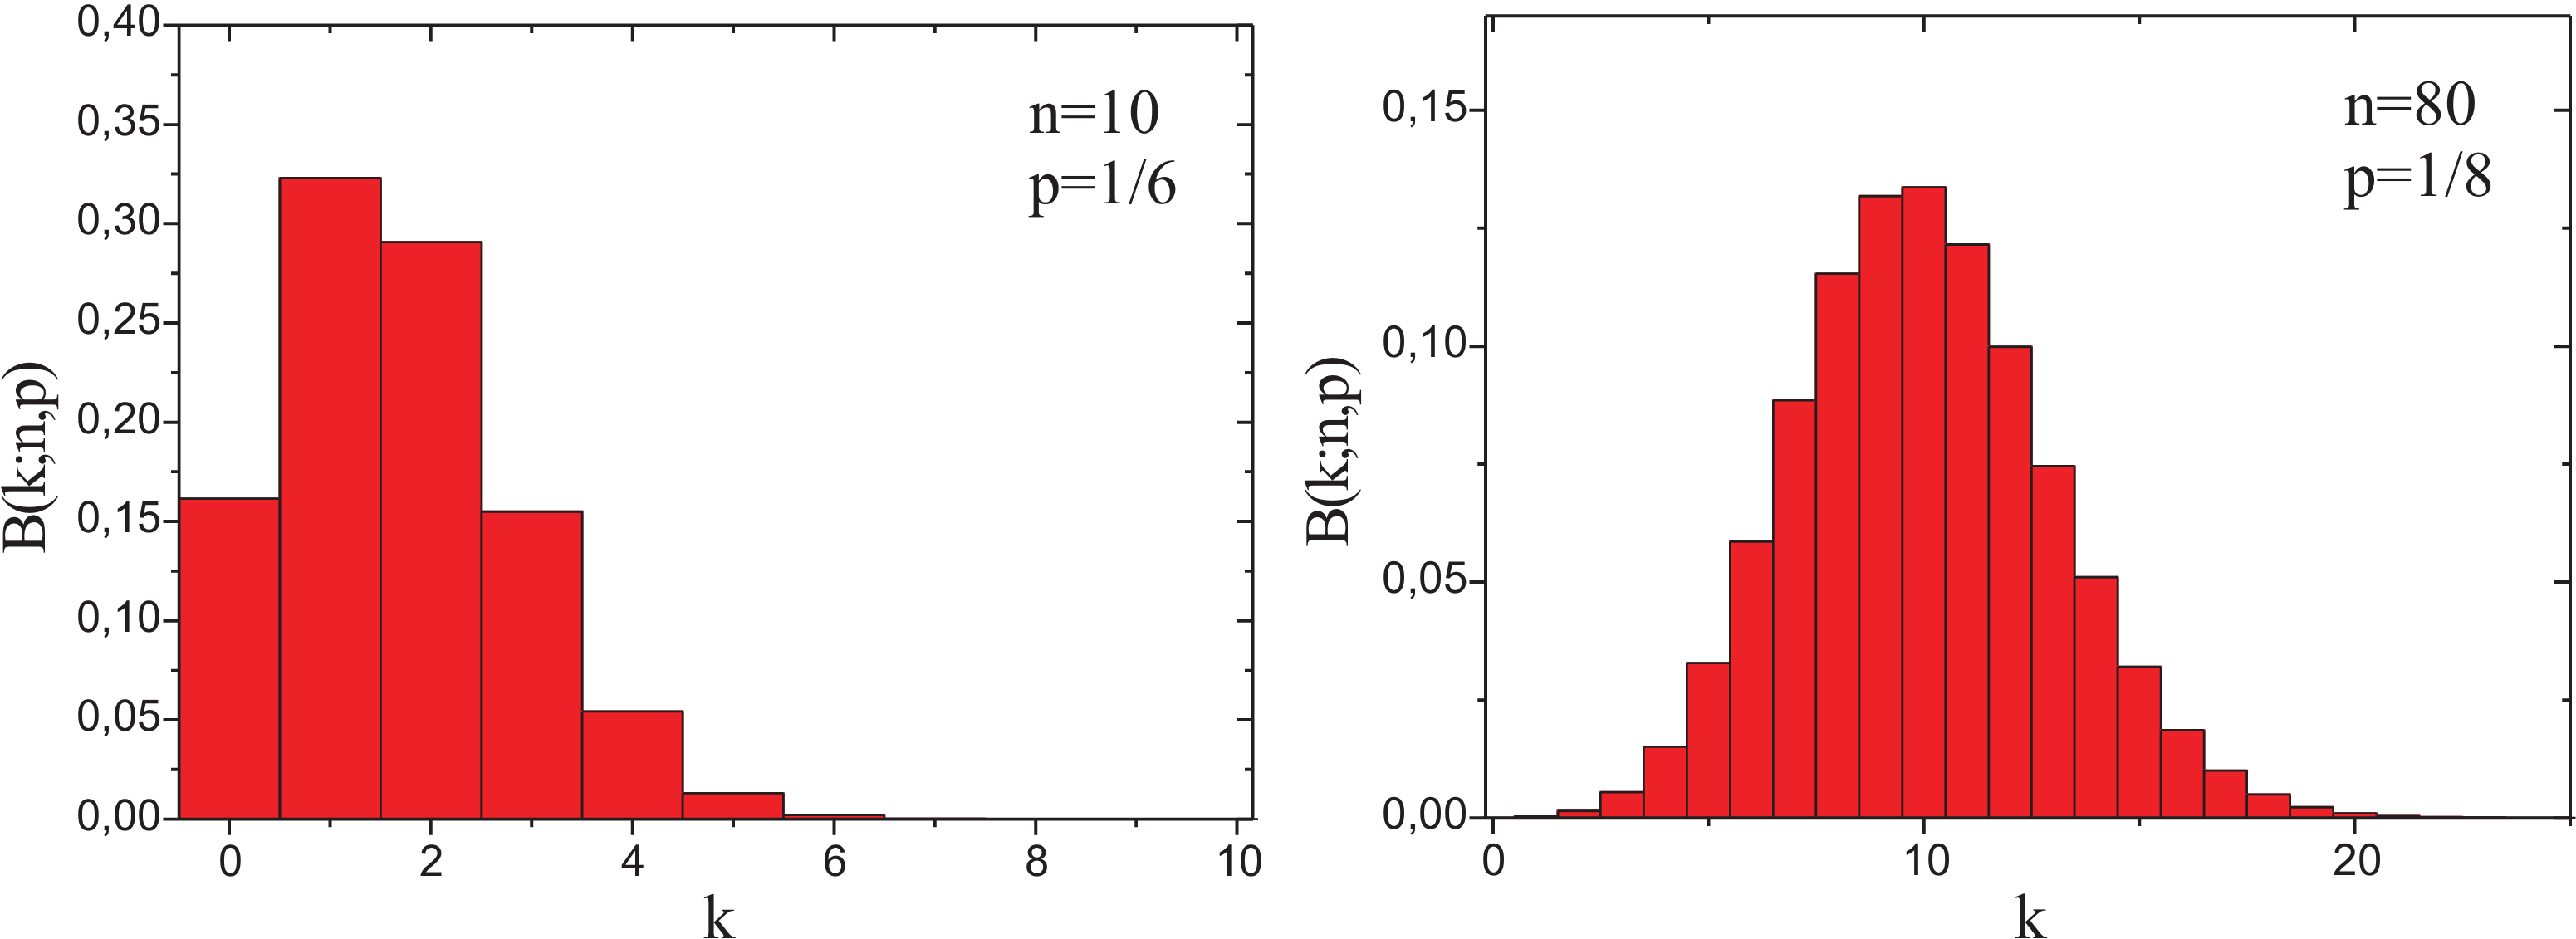
\includegraphics[width=0.9\textwidth]{files/binom_distr_examples.png}
  \caption{Beispiele für Binomialverteilungen}
  \label{fig:binom_distr_examples}
\end{figure}

\textbf{Poissonverteilung.} In vielen Fällen ist die Zahl der betrachteten Atome sehr groß ($n \to \infty$) und die Zerfallswahrscheinlichkeit $(p \to 0)$ sehr klein. Mit diesen Grenzüberlegungen kann, unter Beachtung, dass der Mittelwert endlich ist, von der Binomial- zu einer Poissonverteilung übergegangen werden. Die Wahrscheinlichkeitsverteilung diese ist gegeben durch
\begin{align}
  P(k;\mu) = \frac{\mu^k \e{-\mu}}{k!}. \label{eq:poisson_distr}
\end{align}
Auch hier gilt, dass $k \in \N$. Weiter sind die statistischen Eigenschaften gegeben durch
\begin{align}
  \text{Mittelwert: }& \mean{k} = \mu,\\[0.6em]
  \text{Varianz: }& \sigma^2 = \mu.
\end{align}
Aus der Tatsache, dass $\sigma = \sqrt{\mu}$ ergibt sich das $\sqrt{N}$-Gesetz, welches für die Fehlerbestimmung von gezählten Größen genutzt wird. Für $\mu < 1$ ist die Poissonverteilung in $k$ monoton fallend, besitzt kein Maximum und der wahrscheinlichste Wert ist stets $0$. Für $\mu > 1$  besitzt die Verteilung ein Maximum, dessen Breite durch $\sigma^2$ gegeben ist.

\begin{figure}[H]
  \centering
  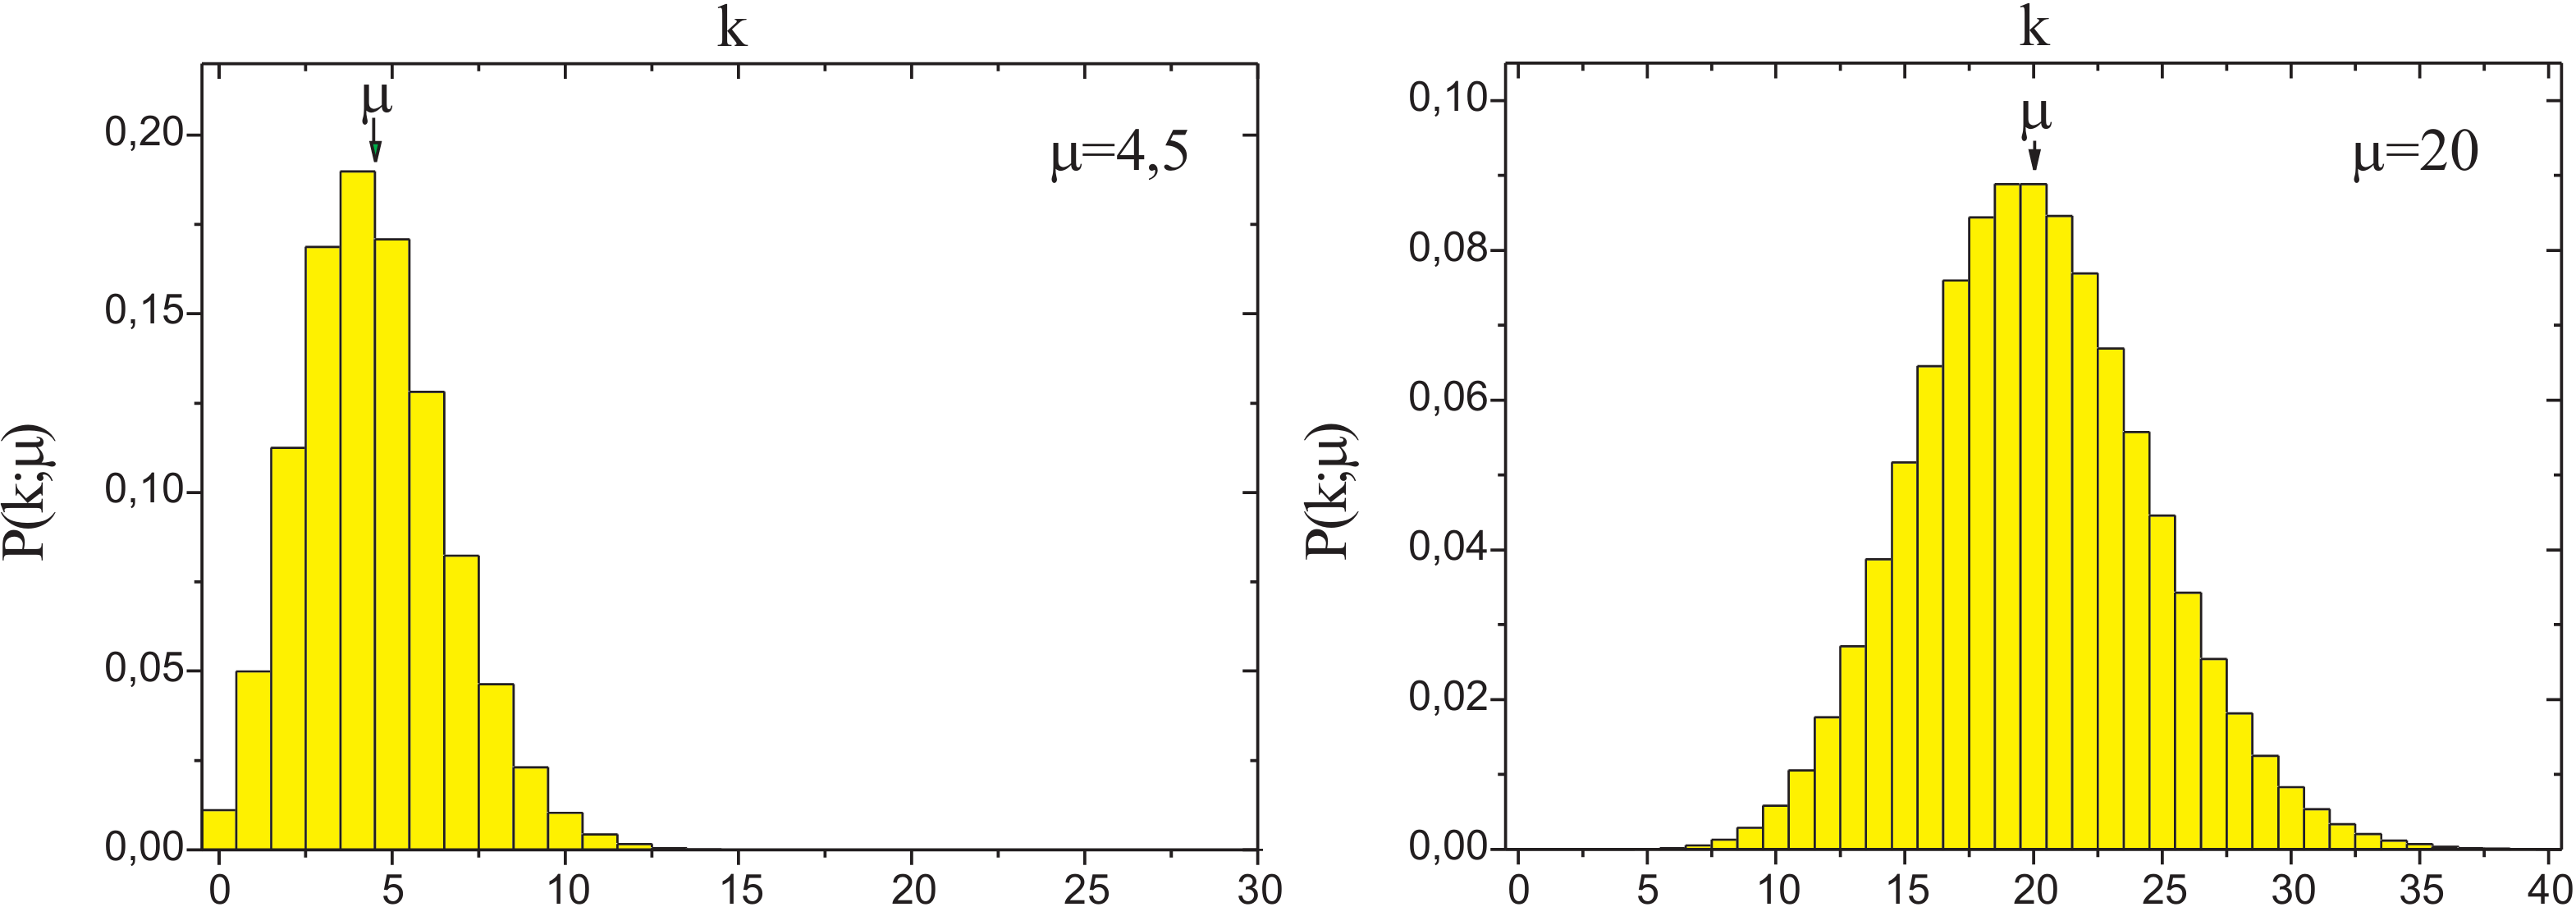
\includegraphics[width=0.9\textwidth]{files/poisson_distr_examples.png}
  \caption{Beispiele für Poisson-Verteilungen}
  \label{fig:poisson_distr_examples}
\end{figure}

\textbf{Gauß-Verteilung.} Um das Maximum ist die Poissonverteilung für kleine Mittelwerte stark asymmetrisch. Mit steigendem $\mu$ nimmt sie eine zunehmend symmetrische Form an und kann für große Mittelwerte ($\mu > 30$) schließlich mit der Gauß-Verteilung approximiert werden. Die allgemeine Verteilungsfunktion der Gauß-Verteilung lautet
\begin{align}
  G(k;\mu,\sigma) = \frac{1}{\sqrt{2\pi} \sigma}\e{-\frac{(\mu - k)^2}{2\sigma^2}}, \label{eq:gauss_distr}
\end{align}
wobei nun $k \in \R$ gilt, es sich also um eine kontinuierliche Verteilung handelt. Mittelwert und Varianz sind hier bereits durch $\mu$ und $\sigma^2$ in der Verteilungsfunktion angegeben. Bekannterweise gibt $\mu$ die Position des Maximums an, während $\sigma$ die Breite der Verteilung angibt.

\begin{figure}[H]
  \centering
  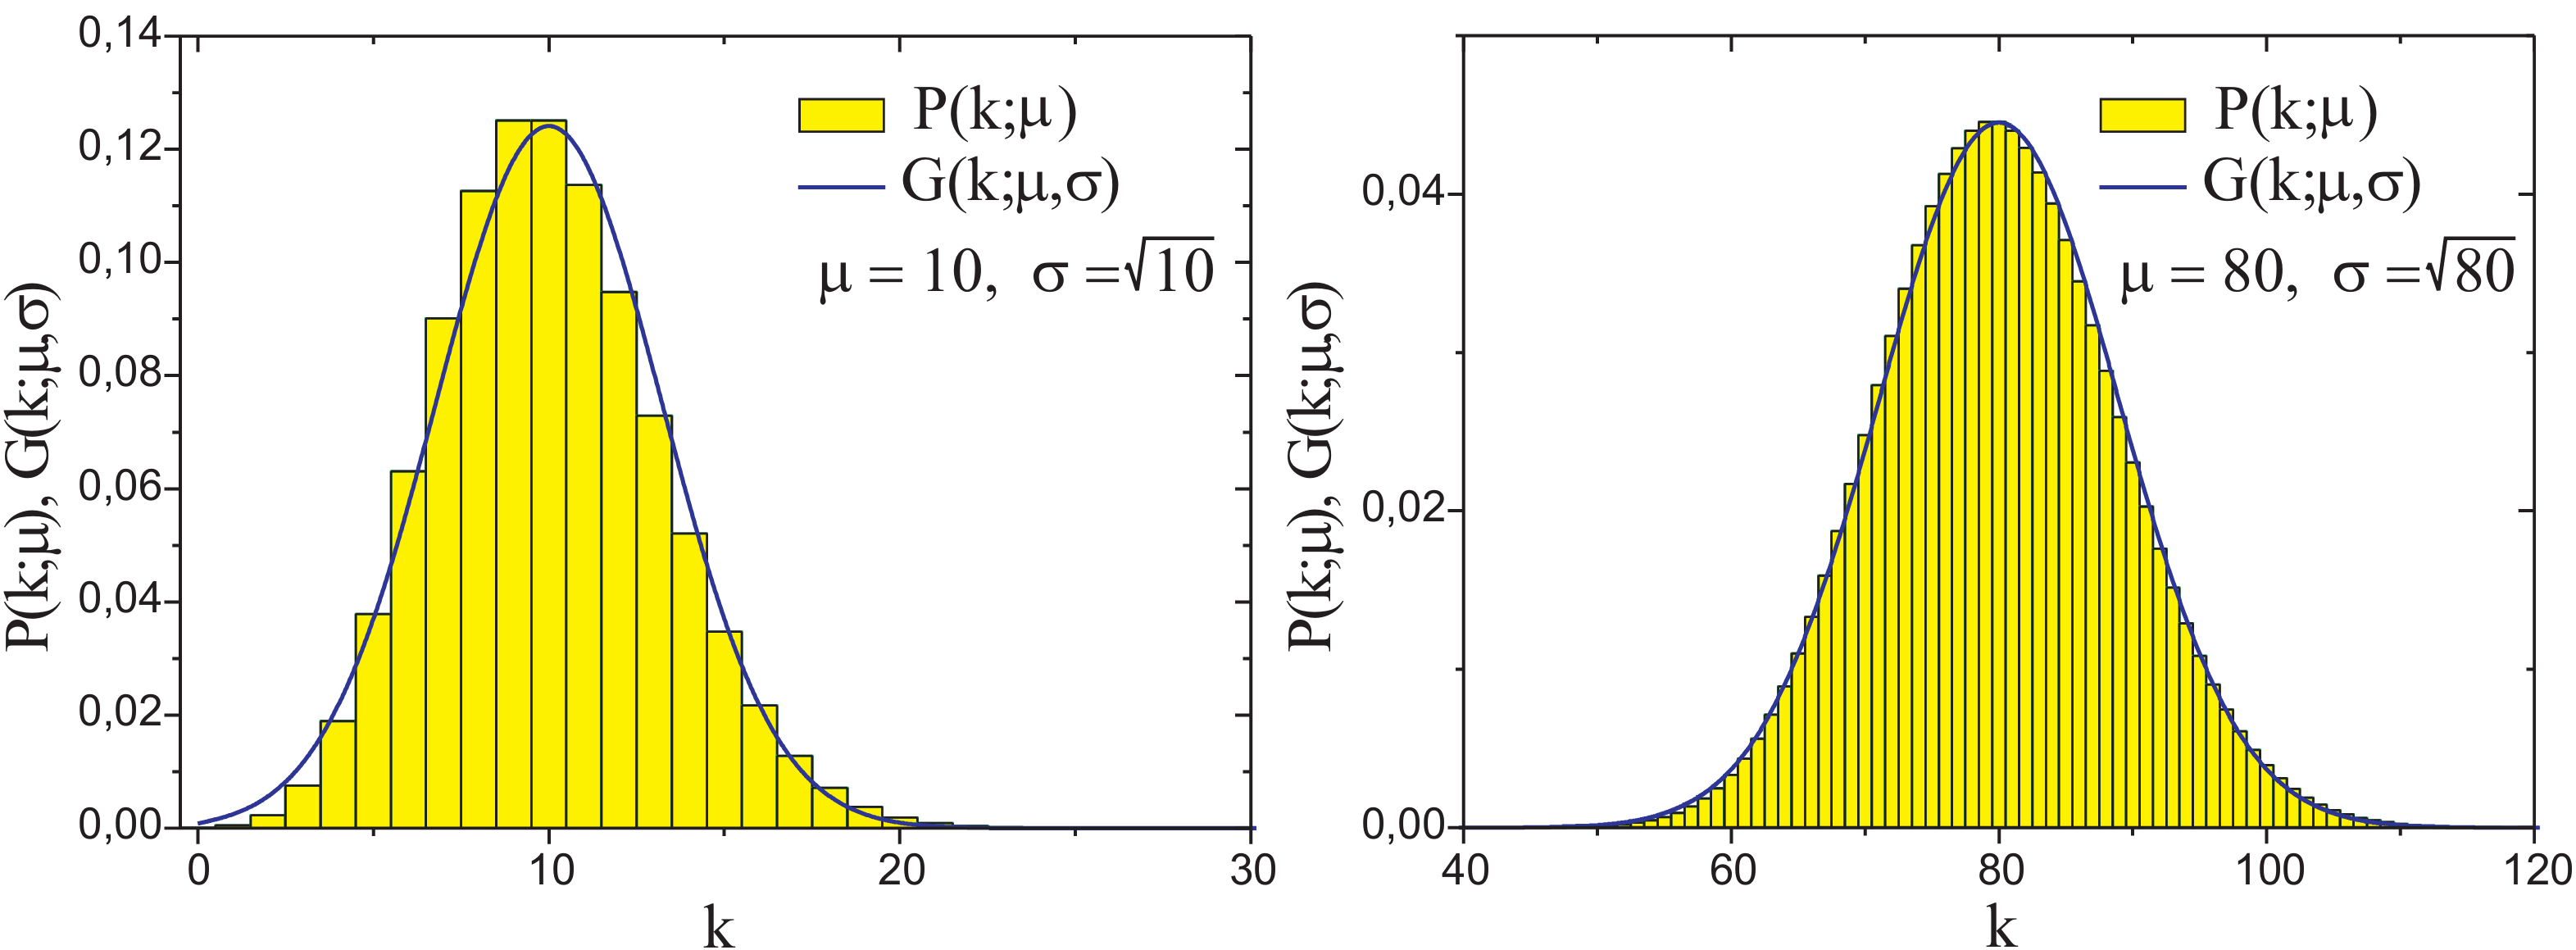
\includegraphics[width=0.9\textwidth]{files/gaus_distr_examples.png}
  \caption{Beispiele für Gauß-Verteilungen}
  \label{fig:gaus_distr_examples}
\end{figure}


\subsection{Versuchsdurchführung}

Im ersten Teil des Versuchs werden wir uns mit der Kalibierung des Zählrohrs beschäftigen und den Plateaubereich untersuchen. Im zweiten Teil nehmen wir Daten auf, um die Statistik der radioaktiven Zerfälle bei großer und kleiner mittlerer Ereigniszahl zu untersuchen. Als radioaktives Präparat wird im ganzen Versuch der $\beta$-Strahler Kobalt-60 ($^60\mathrm{Co}$) verwendet.

\textbf{Bestimmung der Zählrohrcharakeristik.} Ab einer angelegten Einsatzspannung $V_E$ beginnt das Zählrohr, eingehende Strahlung zu registrieren. Um den Plateaubereich zu bestimmen, wird die Spannung ausgehend von $V_E$ um $150\unit{V}$ in Schritten von $25\unit{V}$ erhöht und jeweils die Anzahl der Ereignisse pro 30 Sekunden erfasst. Durch die Untersuchung der Zählraten lässt sich der Plateaubereich und die optimale Spannung $U_0$ für den weiteren Betrieb bestimmen.

\textbf{Untersuchung des Plateauanstiegs.} Innerhalb des Plateaubereichs sollte die Zählrate nicht von der Zählrohrspannung abhängig sein. Um dies zu verifizieren, wird die Probe direkt vor dem Zählrohr platziert und die Zähl-raten je zweimal für eine Minute und zweimal für drei Minuten bei $U_0$ und $U_0 + 100 \si{V}$ gemessen.

\textbf{Verifizierung der statistischen Natur des radioaktiven Zerfalls.} Für diesen Versuchsteil wird das Präparat so platziert, dass ca. 140 bis 150 Zerfälle pro Sekunde registriert werden. In Intervallen von 500ms (entspricht der Torzeit) werden nun für mindestens 2000 Male die Anzahl der Zerfälle des Präparats bestimmt und in ein Histogramm eingetragen.

\textbf{Vergleich der Poisson- und Gauß- Verteilung bei sehr kleinen Zählraten.} Das Präparat wird nun so platziert, dass ca. 40 bis 50 Zerfälle pro Sekunde registriert werden. Bei einer Torzeit von 100ms werden 5000 Messungen durchgeführt und ebenfalls in ein Histogramm eingetragen. 